\documentclass[compress]{beamer}
\usepackage{ifthen,verbatim}

\title{Muon alignment update: full procedure results}
\author{Jim Pivarski, Alexei Safonov}
\institute{Texas A\&M University}
\date{ 6 December, 2007}

\newcommand{\isnote}{}
\xdefinecolor{lightyellow}{rgb}{1.,1.,0.25}
\xdefinecolor{darkblue}{rgb}{0.1,0.1,0.7}
\xdefinecolor{greyone}{rgb}{0.6,0.6,0.6}
\xdefinecolor{greytwo}{rgb}{0.4,0.4,0.4}
\xdefinecolor{greythree}{rgb}{0.2,0.2,0.2}
\xdefinecolor{greyfour}{rgb}{0.1,0.1,0.1}

%% Uncomment this to get annotations
%% \def\notes{\addtocounter{page}{-1}
%%            \renewcommand{\isnote}{*}
%% 	   \beamertemplateshadingbackground{lightyellow}{white}
%%            \begin{frame}
%%            \frametitle{Notes for the previous page (page \insertpagenumber)}
%%            \itemize}
%% \def\endnotes{\enditemize
%% 	      \end{frame}
%%               \beamertemplateshadingbackground{white}{white}
%%               \renewcommand{\isnote}{}}

%% Uncomment this to not get annotations
\def\notes{\comment}
\def\endnotes{\endcomment}

\setbeamertemplate{navigation symbols}{}
\setbeamertemplate{headline}{\includegraphics[height=1 cm]{../cmslogo} \hspace{0.1 cm} \includegraphics[height=1 cm]{../tamulogo} \hfill
\begin{minipage}{5.5 cm}
\vspace{-0.75 cm} \small
\begin{center}
\ifthenelse{\equal{\insertpagenumber}{1}}{}{\textcolor{blue}{\insertsection}}
\end{center}
\end{minipage} \hfill
\begin{minipage}{4.5 cm}
\vspace{-0.75 cm} \small
\begin{flushright}
\ifthenelse{\equal{\insertpagenumber}{1}}{}{Jim Pivarski \hspace{0.5 cm} \insertpagenumber\isnote/\pageref{numpages}}
\end{flushright}
\end{minipage}\mbox{\hspace{0.2 cm}}}

\begin{document}
\frame{\titlepage}

%% \begin{notes}
%% \item This is the annotated version of my talk.
%% \item If you want the version that I am presenting, download the one
%% labeled ``slides'' on Indico (or just ignore these yellow pages).
%% \item The annotated version is provided for extra detail and a written
%% record of comments that I intend to make orally.
%% \item Yellow notes refer to the content on the {\it previous} page.
%% \item All other slides are identical for the two versions.
%% \end{notes}

\begin{frame}
\frametitle{Overview}
\begin{itemize}\setlength{\itemsep}{0.5 cm}
\item The key issue in muon alignment: track fits are too flexible!
\item New 9-pass alignment scheme
\item How the parameters were tuned
\item Alignment quality
\end{itemize}
\vfill 
\mbox{ }
\end{frame}

\begin{frame}
\frametitle{Flexibility of track fits}
\begin{columns}
\column{0.75\linewidth}
\begin{itemize}
\item Tracks for alignment need to be somewhat independent of the
hits; that's why we project from the tracker
\item With small Alignment Parameter Errors (APEs), tracks follow the
hits too closely, presumably by assuming scattering between each
station
\item With large APEs, extrapolation from the tracker is
$\mathcal{O}(\mbox{1 cm})$, presumably because the muons really do scatter
\end{itemize}

\column{0.25\linewidth}
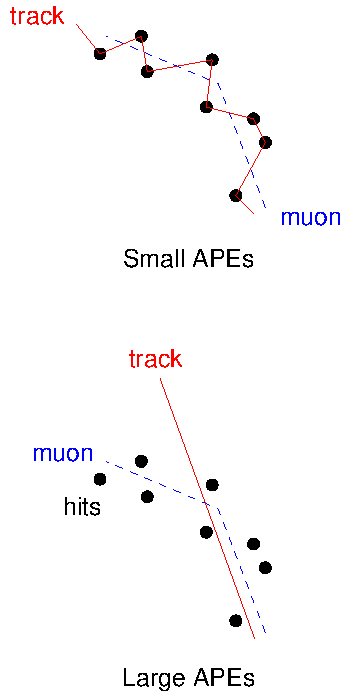
\includegraphics[width=\linewidth]{flexibility.pdf}
\end{columns}

\vspace{0.2 cm}
Potential solutions:
\begin{itemize}
\item \mbox{large APEs, infinite statistics, and hope real scattering is symmetric \hspace{-1 cm}}
\item minimize extrapolations and optimize APEs
\end{itemize}
\end{frame}

\begin{frame}
\frametitle{Method for minimizing extrapolations, using existing tools}

Align one station at a time: e.g.\ for station 2,

\begin{itemize}
\item Set APE = 0 in tracker and station 1
\item Set APE = medium in station 2
\item Set APE = large in stations 3 onward
\item Fit tracks through whole detector, only align station 2
\end{itemize}

\vfill
\textcolor{darkblue}{Pro:} track fit is dominated by extrapolation through only one layer of iron

\vspace{0.1 cm}
\textcolor{darkblue}{Con:} Very CPU intensive

\vfill
Two parameters need to be optimized for most stations: ``medium'' and ``large''
\end{frame}

\begin{frame}
\frametitle{Optimizing APEs}

Simplified to a 1-dimensional case
\begin{itemize}
\item All chambers start 1~cm from the correct position; \\ they need to find their way back to zero
\item If APE is too large, they will spread (large stdev (errorbar))
\item If APE is too small, they will converge too slowly (large mean)
\end{itemize}
\begin{center}
\only<1>{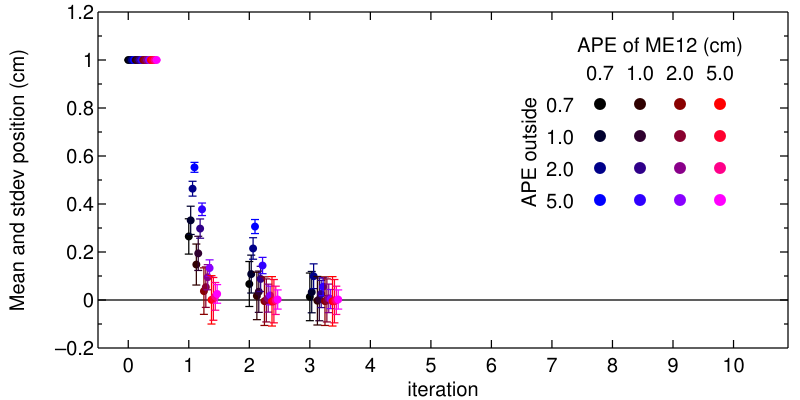
\includegraphics[width=0.8\linewidth]{me12_meanstdev.png}}\only<2>{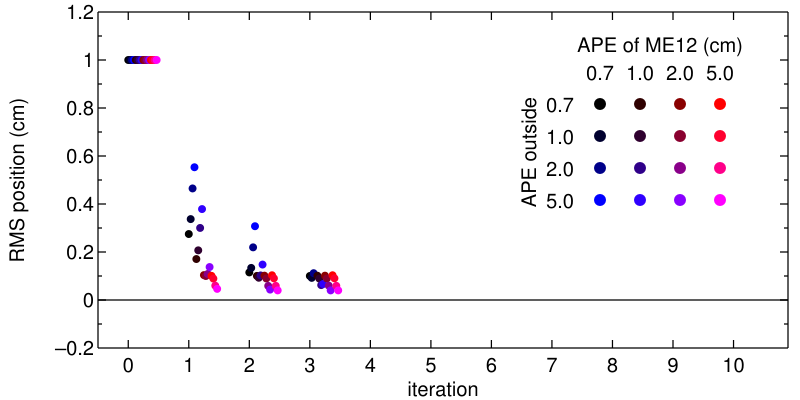
\includegraphics[width=0.8\linewidth]{me12_rms.png}}
\end{center}
\end{frame}

\begin{frame}
\frametitle{Optimized values}

%% ``medium''/``large'' combinations that yield the smallest RMS =
%% $\sqrt{\mbox{mean}^2 + \mbox{stdev}^2}$ (or smallest APE that yields
%% inf~RMS)

\begin{columns}
\column{0.6\linewidth}
\begin{tabular}{c | c c}
& ``medium'' (cm) & ``large'' (cm) \\
& (APE of aligned) & (APE outside) \\\hline
MB1 & 2 & 5 \\
MB2 & 0.5 & 0.5 \\
MB3 & 0.5 & 0.5 \\
MB4 & 0.7 & \\
ME1/1 & 0.5 & 0.5 \\
ME1/2 & 5 & 5 \\
ME1/3 & 0.5 & 0.5 \\
ME2/1 & 0.5 & 0.5 \\
ME2/2 & 0.7 & 0.7 \\
ME3/1 & 0.5 & 0.5 \\
ME3/2 & 0.7 & \\
ME4/1 & 0.5 & \\
\end{tabular}

\column{0.5\linewidth}
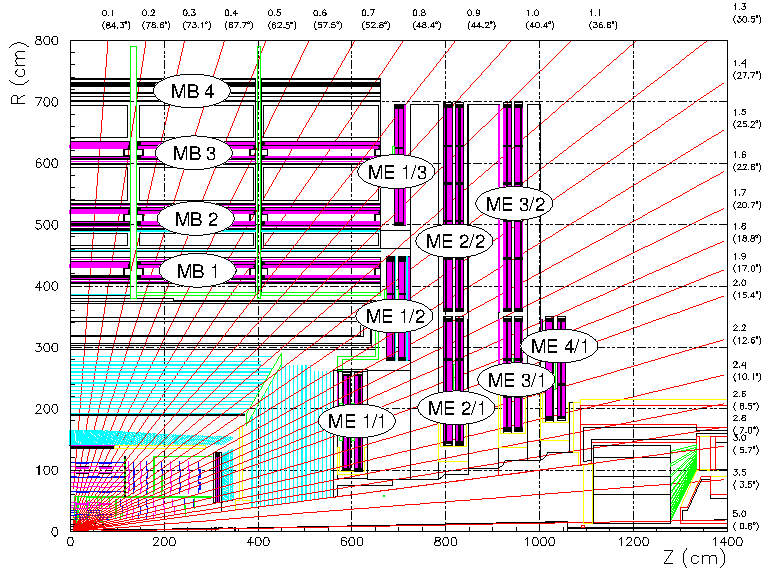
\includegraphics[width=\linewidth]{muon_system_labeled.pdf}
\end{columns}
\end{frame}

\begin{frame}
\frametitle{Which degrees of freedom?}

\begin{itemize}\setlength{\itemsep}{0.25 cm}
\item With 6-dof misalignments, we want to align as many degrees of freedom as possible

\item Constraints:
\begin{itemize}
\item MB1--3 measures $z$ and $\phi_x$ worst, unclear which
\item MB4 does not measure $y$ or $\phi_x$ at all
\item ME measures $\phi_x$ worst, then unclear between $z$ and $\phi_y$
\end{itemize}

\item 8 parameter combinations to try in the barrel, 6 in the endcap

\item Tested all combinations with TeV track resolution

\item \mbox{Marginal best case: let everything float (except MB4 $y$ and $\phi_x$) \hspace{-1 cm}}

\item But ME $z$ and $\phi_x$ distributions were not improved, so I
chose to fix them, too
\end{itemize}

\end{frame}

\begin{frame}
\frametitle{Full procedure}

Each pass has 5 iterations

\begin{enumerate}
\item Align superstructures: wheels and disks
\item Pass 1: align MB1 and ME1/1 (large APEs: 2--5~cm)
\item Pass 2: align MB2 and ME1/2 (small APEs: 0.5--0.7~cm)
\item Pass 3: align MB3 and ME2/1
\item Pass 4: align MB4 and ME1/3
\item Pass 5: align ME2/2 and ME3/1
\item Pass 6: align ME3/2 and ME4/1
\item ``Stage 3'': re-align everything with 500~$\mu$m APEs
\item ``Stage 4'': re-align everything but MB1, ME1/1, and ME1/2 (first step in the muon system) to improve relative alignments
\end{enumerate}
\end{frame}

\begin{frame}
\frametitle{Test for alignment quality}

\begin{itemize}\setlength{\itemsep}{0.1 cm}
\item Using 66000 muons from 10~pb$^{-1}$ of $W$ decays \\ (85\% of the muons from $W$ and $Z$ combined)
\item Starting with complete misalignment: $\pm$5~mm, $\pm$5~mrad at all levels (chamber and wheel/disk)
\item Includes known layer misalignments in CSCs (which we won't improve with this procedure)
\item Two cases:
\begin{itemize}
\item Ideal tracker
\item 10~pb$^{-1}$ misaligned tracker
\end{itemize}
\item Two methods to judge quality:
\begin{itemize}
\item Dimuon resolution for 3.5~TeV Z' (where muon alignment matters most)
\item Stdev of local $x$ (global $r\phi$) residual misalignment, for each station
\end{itemize}
\end{itemize}
\end{frame}

\begin{frame}
\frametitle{\only<1>{Ideal}\only<2>{Misaligned} tracker case}
Dashed line: perfect muon system alignment (best-case goal)

Grey line: official 10 pb$^{-1}$ scenario (not a mean)

\vfill
\only<1>{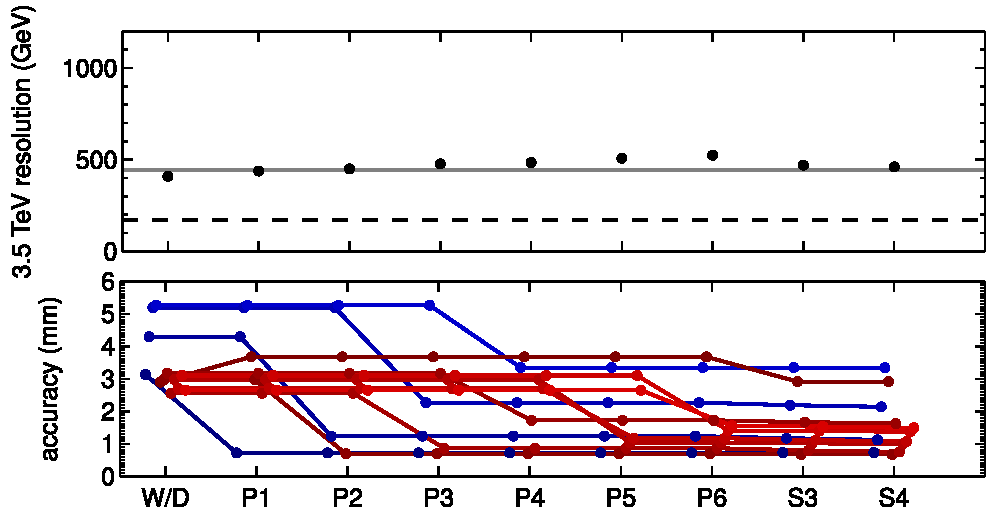
\includegraphics[width=\linewidth]{ideal_tracker.pdf}}\only<2>{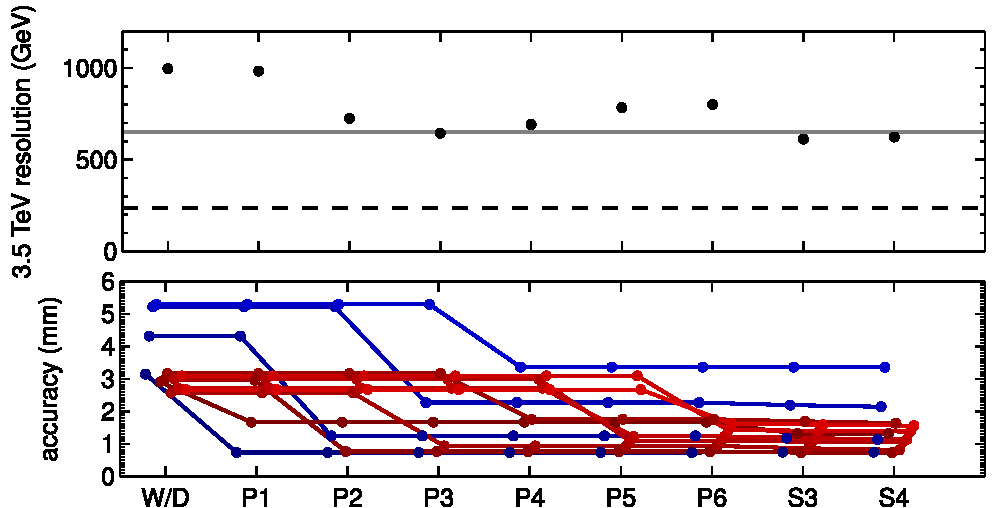
\includegraphics[width=\linewidth]{misaligned_tracker.pdf}}

\vfill
\textcolor{red}{Reds:} endcap stations, \textcolor{blue}{Blues:} barrel stations
\end{frame}

\begin{frame}
\frametitle{Shown as a dimuon spectrum (\only<1>{ideal}\only<2>{misaligned} tracker case)}
\begin{center}
\only<1>{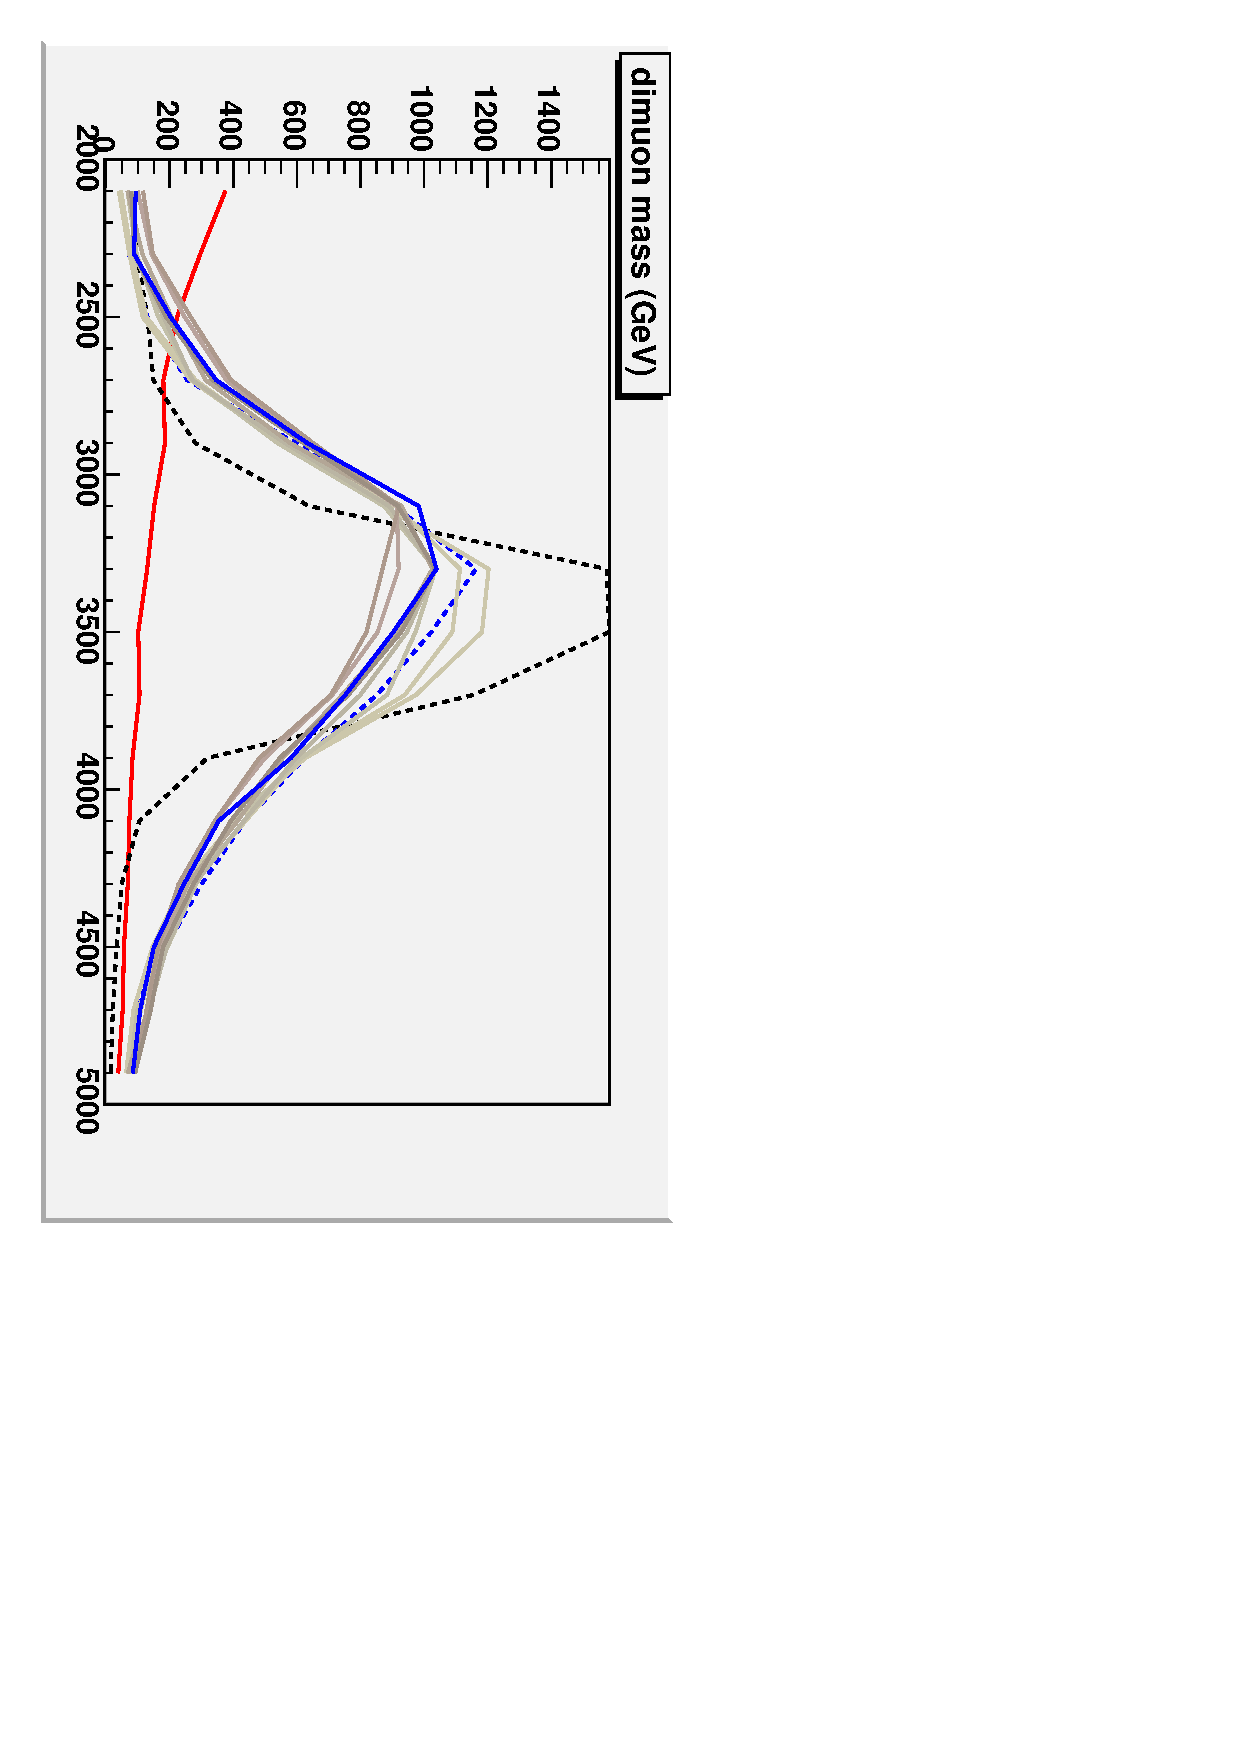
\includegraphics[height=0.8\linewidth, angle=90]{all_superimposed_ideal.pdf}}\only<2>{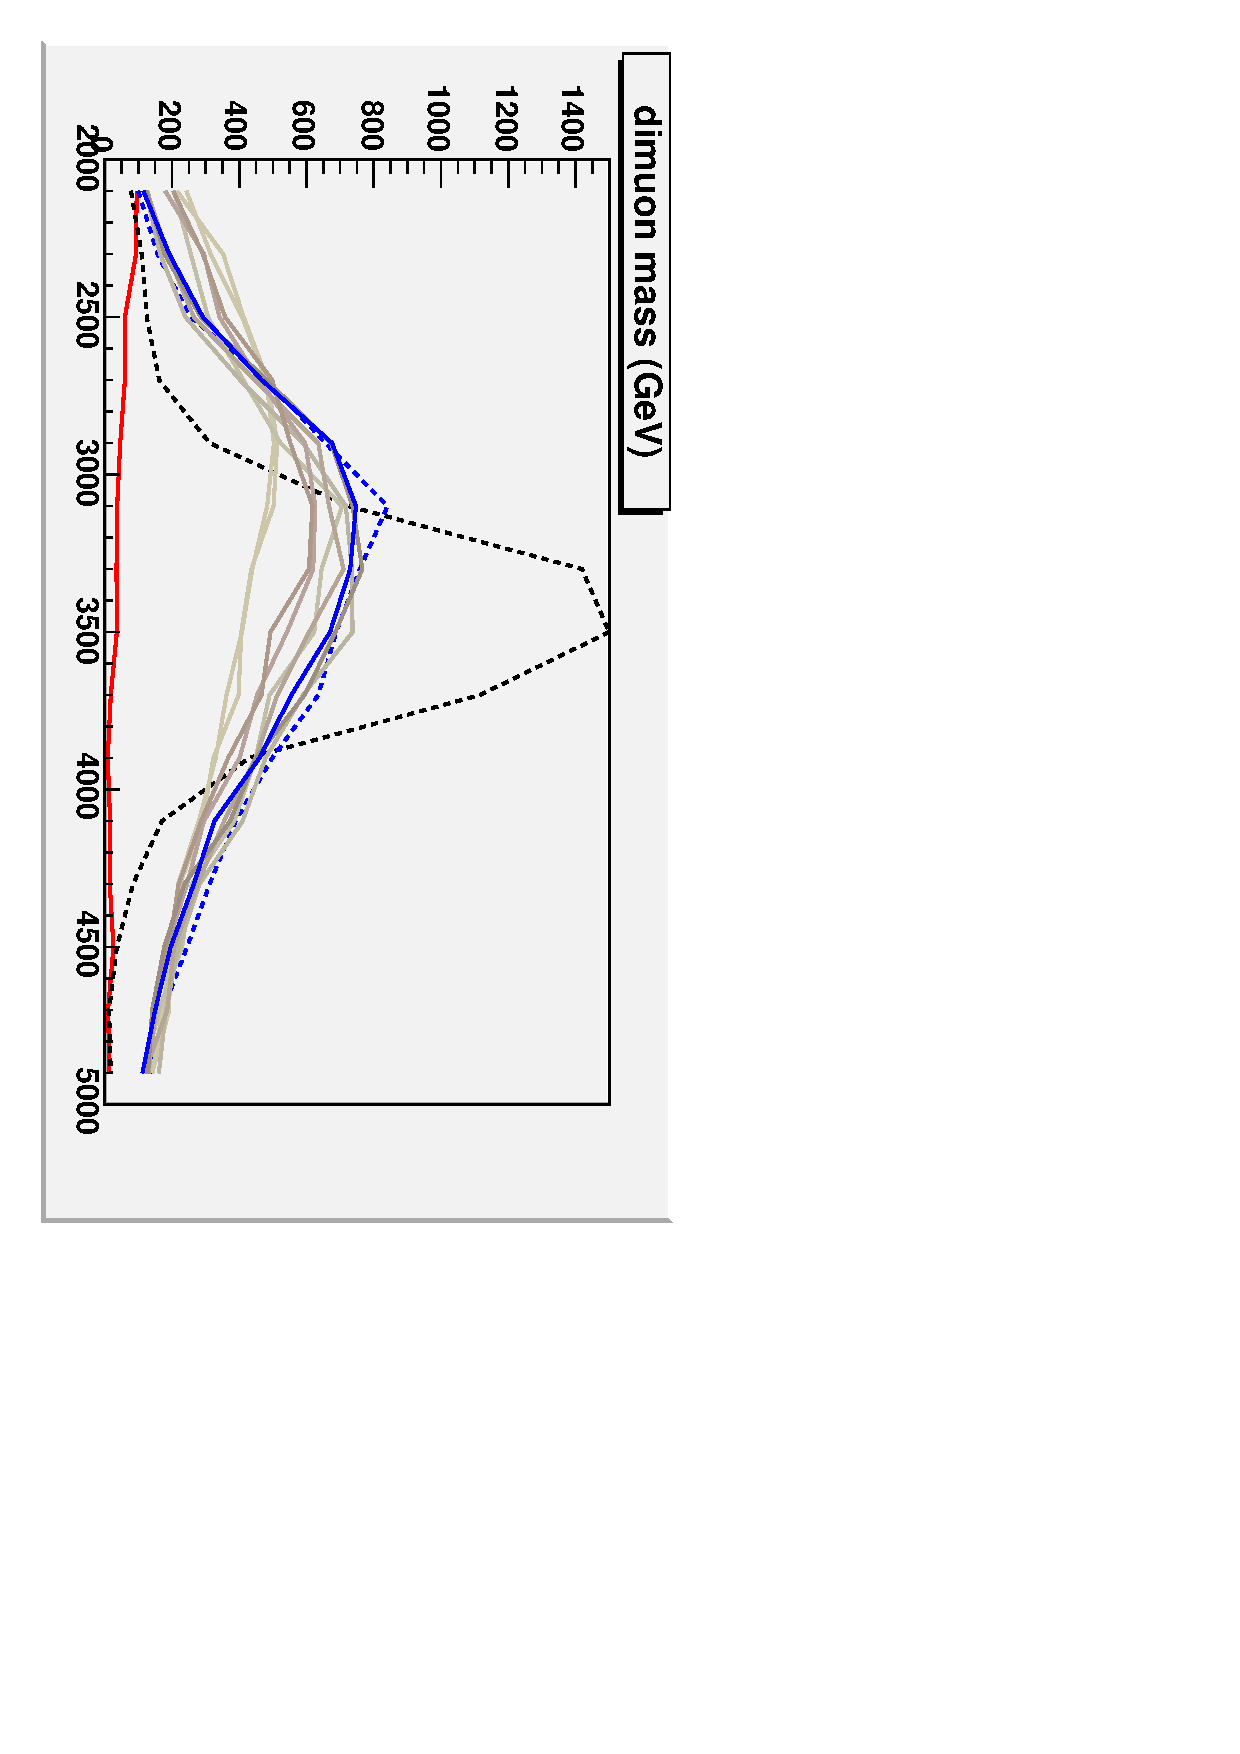
\includegraphics[height=0.8\linewidth, angle=90]{all_superimposed.pdf}}
\end{center}

\vfill \textcolor{red}{Red:} before alignment (peaks at 1~TeV)

\textcolor{greyone}{Darkening} \textcolor{greytwo}{shades} \textcolor{greythree}{of} \textcolor{greyfour}{gray:} alignment passes, ending in \textcolor{blue}{blue}

\textcolor{blue}{Dashed blue:} official 10~pb$^{-1}$ scenario

Dashed black: perfect muon system alignment
\end{frame}

\begin{frame}
\frametitle{Inverted hierarchy?}

\begin{itemize}\setlength{\itemsep}{0.5 cm}
\item Wheels and disks are better aligned than the chambers

\begin{itemize}\setlength{\itemsep}{0.2 cm}
\item wheel/disk (after first pass): 1~mm in $x$ and $y$, 0.3~mrad in $\phi_z$ \\ (corresponds to 0.4--2.5~mm in $r\phi$)
\item chambers (after all passes): 0.7--3.2~mm in $r\phi$
\end{itemize}

\item Official scenario has the opposite: 2--3~mm wheel/disks and 0.5~mm chambers

\item Our method is particularly good at aligning large structures
globally, we need to work on chambers within stations

\end{itemize}
\end{frame}

\begin{frame}
\hspace{-0.83 cm} \textcolor{darkblue}{\Large Other tests in progress}

\begin{itemize}\setlength{\itemsep}{0.2 cm}

\item Robustness: same procedure with a statistical ensemble of 8
starting scenarios (are we looking at a lucky case?)

\item Full scale: 100~pb$^{-1}$

\item Simplification: replace pass1 -- pass6 with a single pass that
aligns all stations at once (to see if those extra steps are helping at all)

\end{itemize}

\vfill
\hspace{-0.83 cm} \textcolor{darkblue}{\Large Ideas for improving the algorithm}

\begin{itemize}\setlength{\itemsep}{0.2 cm}
\item If 10$\times$ statistics improves by $\sqrt{10}$, we will try as many QCD muons as possible

\item Use CSC overlaps to align chambers locally? (requires modifications to the track-fitter)

\end{itemize}
\end{frame}

\begin{frame}
\frametitle{Conclusions}
\begin{itemize}\setlength{\itemsep}{0.5 cm}

\item Post-bugfix, this is the first fully realistic test of the system

\item We want to improve the performance

\item But this is a demonstration that we can at least reach the
standard set by the official scenarios

\end{itemize}

\vfill \mbox{ }

\label{numpages}
\end{frame}

\end{document}
